\documentclass[oneside,final,14pt,a4paper]{extreport}

% set the compiler XeLatex to use fontspec package
% \usepackage{fontspec}
% \setmainfont[Mapping=tex-text]{Times New Roman}
\usepackage{tempora}

\usepackage{vmargin}
\setpapersize{A4}
\setmarginsrb{2.5cm}{2.2cm}{2.2cm}{2.2cm}{0pt}{10mm}{0pt}{13mm}
\usepackage{setspace}
\sloppy
\setstretch{1.5}
\usepackage{indentfirst}
\parindent=1.25cm

%%%%% ADDED TO SUPPORT TT BOLD FACES %%%%
\DeclareFontShape{OT1}{cmtt}{bx}{n}{<5><6><7><8><9><10><10.95><12><14.4><17.28><20.74><24.88>cmttb10}{}
\renewcommand{\ttdefault}{pcr}
%%%%% END %%%%%%%%%%%%%%%%%%%%%%%%%%%%%%% 
\usepackage{atbegshi,picture}
\usepackage[T1,T2A]{fontenc}
\usepackage[utf8]{inputenc}
\AtBeginShipout{\AtBeginShipoutUpperLeft{%
  \put(\dimexpr\paperwidth-1cm\relax,-1.5cm){\makebox[0pt][r]{
\includegraphics[width=3cm]{figs/inno}}}%
}}


\usepackage[english]{babel}
\usepackage[backend=biber,style=ieee,autocite=inline]{biblatex}
\bibliography{ref.bib}
\DefineBibliographyStrings{english}{%
  bibliography = {References},}
\usepackage{blindtext}

\usepackage{pdfpages}
\newenvironment{bottompar}{\par\vspace*{\fill}}{\clearpage}
\usepackage{amsmath,amsfonts}
\usepackage{url}

\usepackage{amsthm}
\newtheorem{theorem}{Theorem}
\newtheorem{corollary}{Corollary}
\newtheorem{lemma}{Lemma}
\newtheorem{proposition}{Proposition}
\theoremstyle{definition}
\newtheorem{definition}{Definition}
\theoremstyle{remark}
\newtheorem*{remark}{Remark}
\theoremstyle{remark}
\newtheorem*{example}{Example}


\usepackage{titlesec}
\usepackage{float}
\usepackage{graphicx}
\graphicspath{{figs/}} %path to images
\usepackage{array}
\usepackage{multirow,array}
\usepackage{caption}
\usepackage{subcaption}
% \usepackage{hyperref}
\usepackage{paralist}
\usepackage{listings}
\usepackage{zed-csp}
\usepackage{fancyhdr}
\usepackage{csquotes}
\usepackage{color}
% \usepackage{anyfontsize}
% \usepackage{mathptmx}
% \usepackage{t1enc}
\usepackage{tempora}
\usepackage{chngcntr}
\usepackage{upgreek} 
\usepackage{bm}
% \usepackage{hyperref}
\usepackage{setspace}
\usepackage{booktabs}
\usepackage{multirow}
\usepackage{longtable}
\usepackage[font=singlespacing, labelfont=bf]{caption}
\usepackage{algorithm}
\usepackage{algpseudocode}
\counterwithout{table}{chapter}
\renewcommand{\thetable}{\Roman{table}}
%Hints
\newcommand\pic[1]{Fig. \ref{#1}} %Ref on figure
\newcommand\tab[1]{Tab. \ref{#1}} %Ref on table

\setlength{\headheight}{32.0976pt}
\usepackage{enumitem}
\newlist{inlinelist}{enumerate*}{1}
\setlist*[inlinelist,1]{%
  label=(\arabic*),
}

\setcounter{secnumdepth}{4}
\captionsetup[table]{labelfont={normalfont}, name={TABLE}, labelsep={newline}}
\counterwithout{table}{chapter}
\renewcommand{\thetable}{\Roman{table}}
\setlength{\parindent}{2em} 
\DeclareCaptionLabelSeparator{figSep}{.\quad}
\captionsetup[figure]{labelfont={normalfont}, name={Fig.}, labelsep=period}
\counterwithout{figure}{chapter}

\titleformat{\section}[hang]{\fontsize{20}{24}\selectfont\filcenter}{\Roman{section}}{1em}{}
\titleformat{\subsection}[hang]{\itshape}{\Alph{subsection}.}{1em}{}[]
\titleformat{\subsubsection}[runin]{\itshape}{\arabic{subsubsection})}{1em}{}[$:$]
\titlespacing{\subsubsection}{1em}{1em}{1em}
\titleformat{\paragraph}[runin]{\itshape}{\alph{paragraph})}{1em}{}[$:$\quad]
\titlespacing{\paragraph}{2em}{1em}{1em}

\pagestyle{fancyplain}

% remember section title
\renewcommand{\chaptermark}[1]%
	{\markboth{\chaptername~\thechapter~--~#1}{}}

% subsection number and title
\renewcommand{\sectionmark}[1]%
	{\markright{\thesection\ #1}}

\rhead[\fancyplain{}{\bf\leftmark}]%
      {\fancyplain{}{\bf\thepage}}
\lhead[\fancyplain{}{\bf\thepage}]%
      {\fancyplain{}{\bf\rightmark}}
\cfoot{} %bfseries


\newcommand{\dedication}[1]
   {\thispagestyle{empty}
     
   \begin{flushleft}\raggedleft #1\end{flushleft}
}
\newcommand\todo[1]{\textcolor{red}{#1}}
\newcommand\temp[1]{\textcolor{blue}{#1}\\}

\usepackage[hidelinks]{hyperref}

\usepackage{tabularx}
\newlength{\conditionwd}
\newenvironment{conditions}[1][where:]
  {%
   #1\tabularx{\textwidth-\widthof{#1}}[t]{
     >{$}l<{$} @{${}\quad{}$} X@{}
   }%
  }

\usepackage{tabularray}
\hypersetup{colorlinks=true, allcolors=black, citecolor=black}

\begin{document}

% 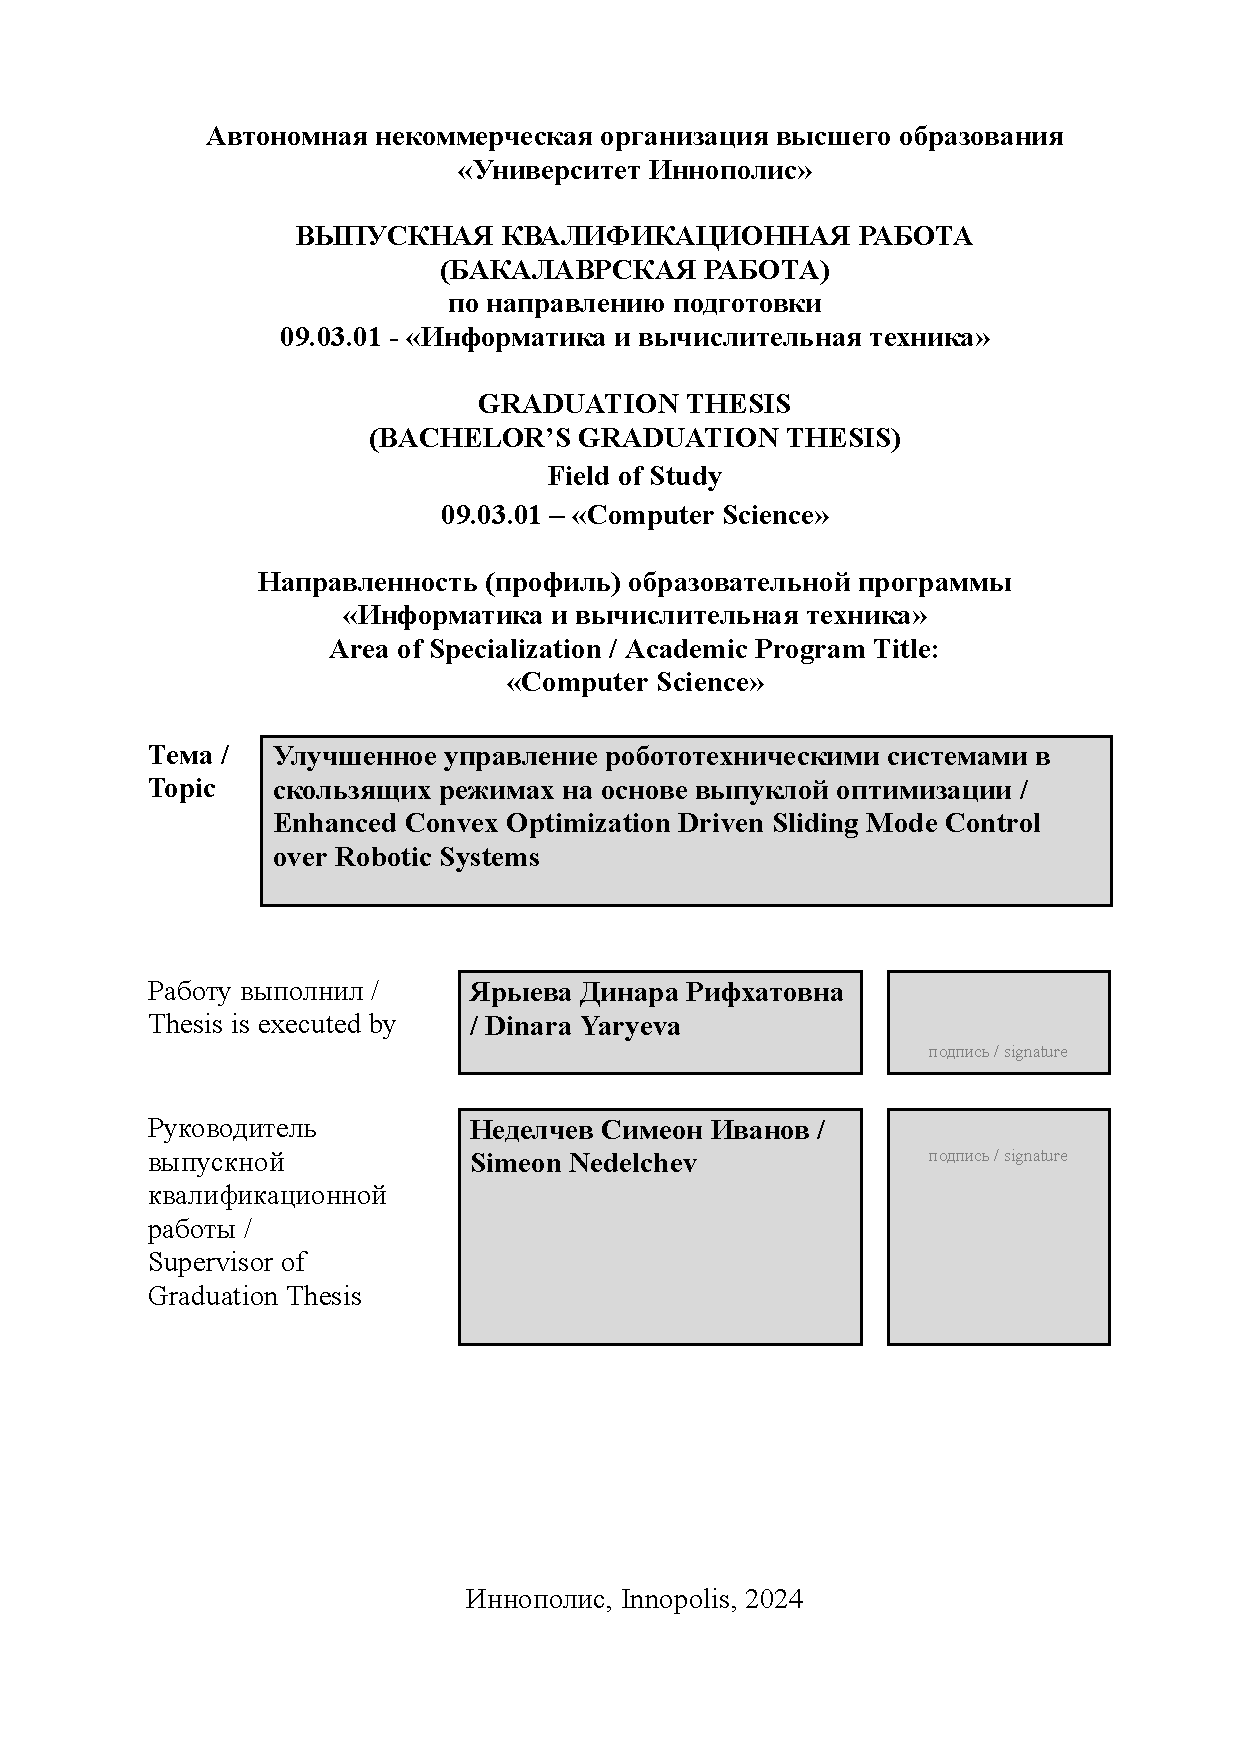
\includepdf[pages=-, offset=75 -75]{title.pdf}
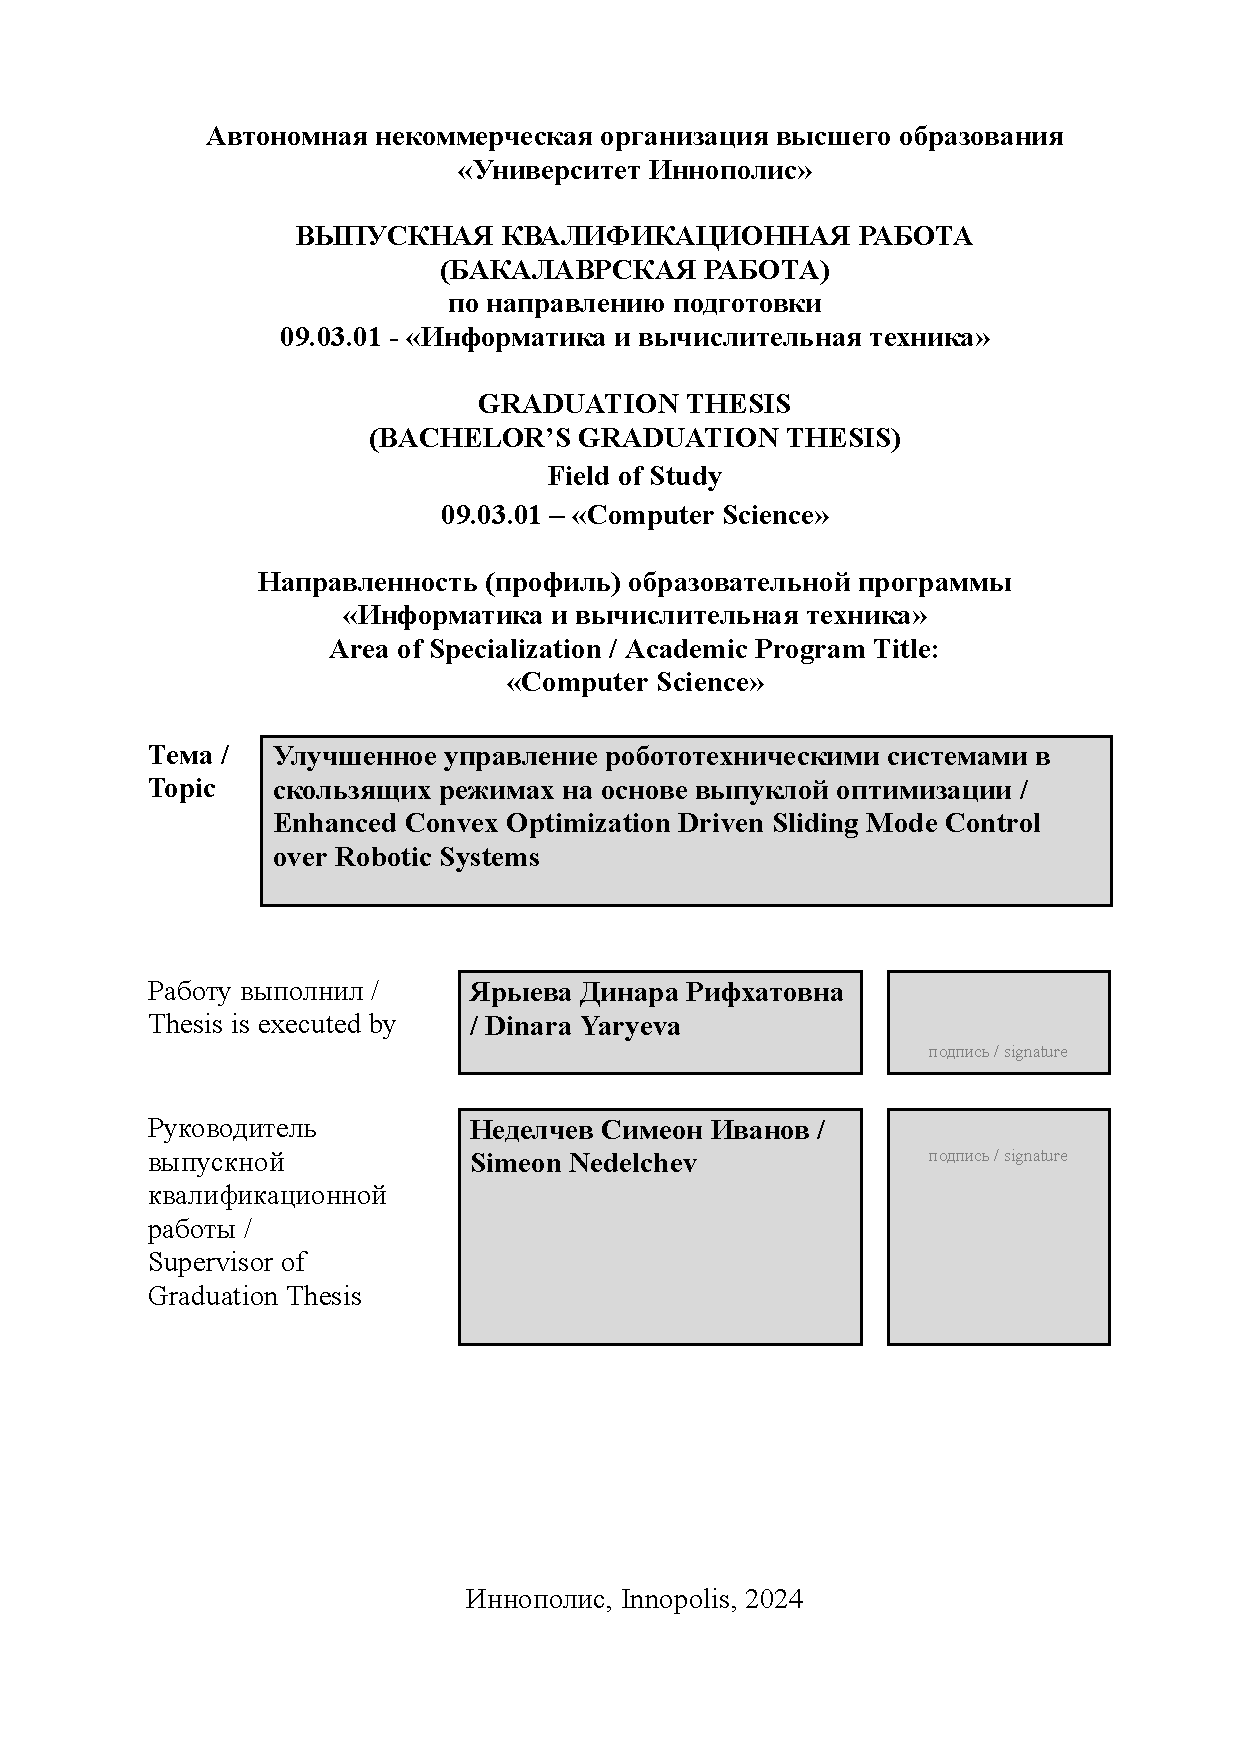
\includepdf[pages=-,offset=25.5mm -25.5mm]{title.pdf}

\tableofcontents
\listoftables
\listoffigures


\newpage
\begin{abstract}
abstract \ldots


\end{abstract}
\setcounter{page}{9} % set manually an actual number from which introduction starts

\chapter{Introduction}

In past robots used to work separately from humans, as most robots were used in fully automated productions without the need for human operator. Nowadays, however, robots work more closely and often in the same space as humans. This subsequently leads to the need to consider the interaction between humans and machines. In many operations both humans and robots can engage in Human-Machine Interactions (HMI), most notably in exoskeletons, robotic hands, haptic interfaces, which are designed to be directly interacting with a human, as well as many others.

While working so closely with these robots in the same space safety becomes a primary concern. Safety is usually achieved through two most common methods as described in \cite{eval_of_safety}:
\begin{enumerate}
    \item design of the robot as well as its actuator;
    \item estimation and control of the force factors in the HMI.
\end{enumerate}
The design of the robot's actuator is vital to the overall safety of the system. Most common drive types tend to have high stiffness, which is a common risk that potentially lead to a mechanical injury in HMI. These drives also often have high impedance and varying transmission ratio, and therefore make robots dangerous in operation. Better impedance and stiffness refine the stability, precision and control accuracy under payload disturbances. This creates a demand for robot drives either with a natural stiffness and a naturally low impedance or with a predetermined way to estimate the external torques and react to them appropriately.

An alternate to the common drives considered in this work, namely the Twisted String Actuator (TSA), has a transmission ratio that decreases overtime resulting in a low impedance and low stiffness. These characteristics render it safe in HMI. Moreover, in this work we will use the TSA as well as consider methods of force factor estimation to ensure safety in HMI.

The most common way to estimate external torques is to install force sensors. However, they significantly increase production costs and the robotic system's weight especially on multiple DOF systems. A much cheaper yet no less effective way - is to implement a sensorless disturbance observer capable of force estimation using only proprioceptive sensors and robot's and actuator's configurations.

While force estimation has been thoroughly studied \cite{collision}, \cite{momentum_obs}, \cite{sliding_mode}, to my knowledge they were not applied to robotic systems based on TSAs. This paper aims to implement various mentioned force estimation algorithms for TSA robotics. The observers are tested on an experimental setup and later compared to determine the most efficient and the most accurate one, hence justifying the importance and novelty of this work.
\chapter{Literature Review}
\label{chap:lr}

\chaptermark{Second Chapter Heading}

This chapter presents a comprehensive overview of existing research on remotely operated vehicles (ROVs),
focusing on modeling and control design. This literature review aims to investigate and synthesize
control strategies, addressing uncertainties from actuator dynamics and environmental factors, which
correspond to the proposed research question.

Section 1 gives a brief description of ROVs, including their types and general attributes.
Section 2 explains the commonly accepted assumptions and mathematical models used in the field.
Section 3 offers an extensive review of various studies on the application of robust control
design for underwater systems. In conclusion, Section 4 summarizes the key insights from the review
and suggests a control methodology.

\section{Overview on ROVs}
\todo{\#TODO Add more sorces and get more info about ROVs.}

    This section provides an overview of ROVs, from their classification and applications to their
    inherent characteristics and challenges. The obtained knowledge forms a basis for ROV modeling
    and control design.

    \temp{ROV physics -> complex model design}
    According to \cite{rov_review}, an ROV's mechanical structure consists of a monitoring camera, a sensor
    for gathering navigation data, and actuators for directional control. A
    comparative study \cite{overview} found that the physical aspects that affect ROV functions are the accuracy of
    sensor systems and the thruster designs. The unpredictable nature of underwater currents, drag,
    and buoyancy dynamics can also have a serious impact on a ROV's performance, complicating model
    design.

    \temp{Small ROVs are more preferrable -> wide range applications}
    A recent systematic review \cite{inspection_review} concluded that there are two primary classifications for ROVs based
    on their functions and intended use: observation class and work class. Observation class vehicles
    are typically small and limited to shallow waters with propulsion power up to a few kilowatts. Work
    class vehicles can perform heavy-duty work, requiring significant hardware
    system complexity. Thus, when the functionality of these large
    ROVs is not necessary, a smaller ROV is preferred for a wide range of applications.

    \temp{Applications of ROV -> control objectives}
    Several studies \cite{rov_review, overview} have identified that ROVs have become crucial for industrial applications,
    offshore oil and gas exploration, patrolling, and surveillance. Therefore, its control system
    should focus on position tracking and station keeping in the presence of parameter and environmental uncertainties, addressing the following issues.

    \todo{\#TODO Add connection to modelling, wrap it up}

\section{Mathematical Modelling}

    Remotely operated vehicles require mathematical models for various purposes, including control
    system design, simulation, and performance analysis.

    \temp{SRB}
    Thor I. Fossen \cite{fossen:guidance} provided a complete description of the fundamentals of mathematical modeling for marine
    vehicles. In his book, ROV was represented as a single rigid body (SRB) by considering 
    it as a solid mass with no internal movement or deformation. The SRB model has drastically simplified the modeling while capturing the essential
    dynamics of the system. 

    \temp{Kinematics and dynamics}
    From a kinematic
    point of view, ROVs have six degrees of freedom (DoFs). However, the orientation expressed
    in the rotation angles could eventually lead to the singularity. To solve this issue,
    \cite{quat_smc} proposed the quaternions representation. The dynamics was derived based on classical
    physics laws: Newton’s Second Law and Euler-Lagrange equation, forming the set of nonlinear equations.
    The study \cite{identification} simplified the equations and represented them in a matrix form.

    \temp{Parameter estimation}
    However, several sources have established that some aspects of the ROV dynamics require empirical
    estimates due to their complex, nonlinear, and coupled nature \cite{fossen:guidance, bluerov}. For instance, the inertia
    of the surrounding fluid cannot be neglected when the vessel moves through a viscous medium. Additionally, water damping is another source of nonlinearity that
    can be approximated as a function of the velocity. Finally, aside from buoyancy and
    gravity, it is common practice to cancel all other forces acting on a vehicle, although it can also impact the dynamics \cite{bluerov}.

    \temp{Thruster modelling}
    Moreover, thruster modeling must be applied to define the desired thrust of each thruster. A recent
    study by \cite{bluerov} stated that creating an accurate thruster model can be challenging due to the
    influence of factors such as motor models, hydrodynamic effects, and propeller mapping.
    
    \temp{Uncertaint model-> control objectives}
    By making these simplifications, the control system cannot independently provide effective control
    over such uncertain dynamics. As a result, a robust controller design is necessary for precise ROV
    position tracking.

\section{Control Solutions}

    \temp{Connect modelling and control}
    Controlling an ROV is a complex task that requires a set of processes to stabilize the vehicle and
    to make it follow the operator's instructions. To ensure the robustness of the system, it is
    necessary to define a control system that can handle disturbances caused by parameter and
    environmental changes. \\
    According to \cite{overview}, there are two main challenges associated with ROVs control:
    \begin{enumerate}
        \item Unmodeled elements like added mass and hydrodynamic coefficients.
        \item Highly nonlinear dynamics of the underwater environment which cause significant disturbances to the vehicle.
    \end{enumerate}

    \temp{Base approach -> SMC}
    The research on ROV control showed several schemes that can achieve robust stability under
    variable disturbances. The classical approach applied is sliding mode control (SMC), which was
    introduced by Slotine \cite{slotine}. SMC is an effective way to address the issues mentioned above and is,
    therefore, a feasible option for controlling underwater vehicles. However,
    standard SMC introduces high-frequency signals, which can cause actuator switching and consequently
    decrease its lifetime.

    \temp{Better SMC variations}
    \todo{\#TODO Change sources and control approaches}\\
    The modern SMC interpretations keep the main advantages,
    thus removing the chattering effects. One of the possible approaches is Adaptive Sliding Mode Control
    (ASMC) design. \cite{fossen:control} designed an effective hybrid control mechanism for the underwater system that
    follows a given route, adapting to dynamic disturbances. \cite{adaptive_smc} improved a control system for ROVs,
    eliminating the need for dynamics linearization. Another way to refine SMC is to add an integral
    component into the controller equation. The proposed Integral Sliding Mode Control (ISMC) reduced
    chattering, effectively eliminating the uncertainty of the model parameters \cite{integral_smc}.

    \temp{My proposal-> use optimization}
    \todo{\#TODO Connect previous part to my proposed control scheme}\\
    The choice of control strategy should be based on the specific
    requirements and characteristics of the underwater vehicle. While both SMC modifications showed
    precise control, these approaches faced certain challenges \cite{integral_smc}, \cite{adaptive_smc}. The ISMC method had limitations in adapting to rapidly changing dynamics, while the ASMC method experienced potential trade-offs in transient performance.
    These problems were opposite to each other. Therefore, combining them into Adaptive Integral Sliding
    Mode Control (ADISMC) can be a good idea to leverage the strengths of both methods and compensate
    for their weaknesses.

\section{Summary}
    \todo{\#TODO Change according to my proposed control scheme}

    This literature review comprehensively examined the general characteristics, mathematical modeling,
    and control solutions for underwater vehicles. This overview identified a gap in the field of robust
    control for remotely operated vehicles, particularly in dealing with parameter and environmental
    uncertainties. While the original sliding mode control scheme provided robust stability, it suffered
    from high-frequency output oscillations. There were several variations of SMC available, and each
    algorithm has its limitations. To address this research gap, a combination of adaptive and integral
    sliding mode modifications was proposed.
\chapter{Mathematical Model}
\label{chap:mat}

\chaptermark{Second Chapter Heading}


\section{Modelling}

    Remotely operated vehicles (ROVs) are complex systems that require mathematical models for various purposes, 
    including control system design, simulation, and performance analysis. With accurate mathematical models, 
    ROVs are able to navigate through different underwater terrains and complete control tasks with a good 
    precision. Also, the simulation, based on these models, are suitable to test different work scenarios and 
    detect undesirable ROV's behaviour before the physical experiment. \\    
    
    The fundamentals of the modelling for marine vehicles were fully described in Fossen().
    Using common assumptions, ROV is treated as a single rigid body with six degrees of freedom (DOF).
    By considering the vehicle as a rigid body, we can simplify the mathematical modeling process while capturing the essential dynamics 
    of the system. \\

    In order to effectively model rigid bodies, it is crucial to consider their kinematic and dynamic properties.\\

    \subsection{Notations}


    Before proceeding to theoretical derivations, it is necessary to clarify the general notations.
    For the motion with six DOF, six independent coordinates are defined in the coordinate frame: 
    three for translational directions (surge, sway, and heave) and three for rotational directions 
    (roll, pitch, and yaw) as depicted in (Fig. \ref{image:6dof})

    \begin{figure}[H]
        \centering\includegraphics*[width=0.5\textwidth]{6dof}
        \caption{6 DOF of a marine vehicle}
        \label{image:6dof}
    \end{figure}

    The linear position is defined as $r = [r_x, r_y, r_z]^\top$ for translation along xyz axis respectively,
    while orientation can be expressed in terms of Euler angles around corresponding axis. 
    But Euler angles will eventually lead to the singularity 
    when sway angle is $± 90^{\circ}$. 
    However, the quaternions can resolve this problem by adding redundancy into the representation. 
    The orientation quaternion is defined in scalar-first form as 
    $q = q_0 + q_1\cdot i + q_2\cdot j + q_3\cdot k = [q_0, q_1, q_2, q_3]^\top$

    For each direction, the velocity vectors can be defined separately: 
    $v = [v_x, v_y, v_z]^\top$ for translation along xyz axis and
    $\omega = [\omega_x, \omega_y, \omega_z]^\top$ for rotation around xyz axis respectively.
    The same applies to linear forces $f$ and torques $\tau$.

    To summarize, the general notations look like:

    \begin{figure}[H]
    \begin{tabular}{ccc}
        \hline Notation & Description & Dimentionality\\
        \hline
        $r$ & Linear position vector & $\in \mathbb{R}^{3}$ \\
        $q$ & Angular position (orientation) vector & $\in \mathbb{R}^{4}$\\
        $v$ & Linear velocity vector & $\in \mathbb{R}^{3}$\\
        $\omega$ & Angular velocity vector & $\in \mathbb{R}^{3}$\\
        $f$ & Vector of linear forces& $\in \mathbb{R}^{3}$ \\
        $\tau$ & Vector of torques& $\in \mathbb{R}^{3}$ \\
        \hline
        \end{tabular}
        \caption{Notation}
        \label{table:notation}
    \end{figure}

    For the convenience, it is desirable to define combined vectors of positions, velocities and forces as:
    $\bar{q} = \left[\begin{array}{ll}
        r \\
        q
    \end{array}\right]$, $\bar{v} = \left[\begin{array}{ll}
        v \\
        \omega
    \end{array}\right]$ and $\bar{f} = \left[\begin{array}{ll}
        f \\
        \tau
    \end{array}\right]$

    In order to manipulate with obtained vectors, it is necessary to define cross product operators:\\
    $S(\lambda)$ is a skew-symmetric matrix defined such that:
    $$
    S(\lambda)=\left[\begin{array}{ccc}
        0 & -\lambda_3 & \lambda_2 \\
        \lambda_3 & 0 & -\lambda_1 \\
        -\lambda_2 & \lambda_1 & 0
    \end{array}\right]
    $$ therefore $S(u)v = u \times v$ for vectors v,u $\in \mathbb{R}^{3}$ \\
    $\bar{\times}^*$ is the $\mathbb{R}^{6}$ cross product operator defined as: \\
    
    $
    \bar{v}\bar{\times}^*=\left[\begin{array}{ll}
        S(\omega) & 0_{3 \times 3} \\
        S(v) & S(\omega)
    \end{array}\right]
    $ where $\bar{v} = \left[\begin{array}{ll}
        v \\
        \omega
    \end{array}\right]$

\subsection{Frames of reference}

    In order to derive the kinematics and dynamics of the system, the calculations need to be projected into 
    the same frame of reference. 
    Sometimes several coordinate frames are defined based on the system configuration. 
    
    For ROV, it is reasonable to define two coordinate frames. 
    These frames are the earth-fixed frame, which is inertial with fixed origin, and the body-fixed frame, 
    which is a moving frame attached to the vehicle. as depicted in (Fig. \ref{image:frames}). 
    \begin{figure}[H]
        \centering\includegraphics*[width=0.5\textwidth]{frames}
        \caption{The frames}
        \label{image:frames}
    \end{figure}

    The origin of the body-fixed frame usually coincides with the vehicle's center of mass,
     and its axes are chosen along the vehicle's principle axes of inertia.

    In further derivations, the state variables of the rigid body expressed in the body-fixed frame would be noted by $^B$ and in the earth-fixed frame by $^N$.

\subsection{Kinematics}

    Kinematics describes the motion of the marine vehicle without considering the forces acting upon it.
    In order to describe kinematic motion of the body, it is necessary to find relation between velocities in two coordinate frames.
    This relation can be represented with linear transformations as:
    $$
    \begin{aligned}
        & \dot{\bar{r}}^N=J(\bar{r}^N) \bar{v}^B \\
        \text{where } & J(\bar{r}^N)=\left[\begin{array}{cc}
        R(\bar{r}^N) & 0_{3 \times 3} \\
        0_{3 \times 3} & T(\bar{r}^N)
        \end{array}\right]
    \end{aligned}
    $$
    where the $R$ is the rotational matrix and the $T$ is the transformation matrix. 
    The kinematic equations for the marine vehicle using quaternions can be written as follows:
    $$
    \begin{aligned}
    & R(q)=\left[\begin{array}{ccc}
        1-2\left(q_2^2+q_3^2\right) & 2\left(q_1 q_2-q_3 q_0\right) & 2\left(q_1 q_3+q_2 q_0\right) \\
        2\left(q_1 q_2+q_3 q_0\right) & 1-2\left(q_1^2+q_3^2\right) & 2\left(q_2 q_3-q_1 q_0\right) \\
        2\left(q_1 q_3-q_2 q_0\right) & 2\left(q_2 q_3+q_1 q_0\right) & 1-2\left(q_1^2+q_2^2\right)
        \end{array}\right]\\
    & T(q)=\frac{1}{2}\left[\begin{array}{rrr}
        -q_1 & -q_2 & -q_3 \\
        q_0 & -q_3 & q_2 \\
        q_3 & q_0 & -q_1 \\
        -q_2 & q_1 & q_0
        \end{array}\right]
    \end{aligned}
    $$

\subsection{Model dynamics}

    The Newton-Euler approach is commonly used to describe the dynamics of marine vehicles.
    This approach relates the applied forces and moments to the vehicle's accelerations and angular accelerations.
    The general equation of motion using the Newton-Euler approach in the body-fixed frame can be written as:
    $$
    M\dot{\bar{v}}^B+\bar{v}^B\bar{\times}^*M\bar{v}^B=\bar{f}^B
    $$
    where $M$ represents the inertia matrix of the rigid body and 
    $\bar{f}$ represents the total force acting on it.\\
    The equation can be transformed into manupulator equation like:
    $$
     M_B \dot{\bar{v}}^B+C_B(\bar{v}^B) \bar{v}^B
    = \bar{f}^B
    $$
    where
    $M_B \in \mathbb{R}^{6 x 6}$ is the rigid body mass matrix,
    $C_B(\bar{v}^B) \in \mathbb{R}^{6 x 6}$ is the rigid body Coriolis and centripetal forces matrix.

    However, additional terms should be included in the equation to determine the specifics of the ROVs model. 
    These terms comprise added mass, which represents the inertia of the surrounding fluid, the shift of the 
    center of buoyancy due to changes in trim and heel angles, and damping effects. 
    By incorporating these terms into the manipulator equation derived from the Newton-Euler approach, 
    the model becomes more accurate and reflects the natural behavior of the ROV.    

\subsection{Center of Gravity and Center of Buyonancy}
    
    Due to the robust design of the marine vehicles, the center of byonancy(COB) is usually alligned with
    the center of mass(COM), but placed higher.
    This shift between centers causes torque acting against the capsize (Fig. \ref{image:scheme}).\\
    \begin{figure}[H]
        \centering\includegraphics*[width=0.5\textwidth]{01_srb}
        \caption{The vehicle scheme}
        \label{image:scheme}
    \end{figure}
    
    If we place the origin of the body frame at the center of mass(COM), the mass matrix can be expressed as:\\
    $$
    M_B=\left[\begin{array}{cc}
        m I_{3 \times 3} & -m S\left(r_G^B\right) \\
        m S\left(r_G^B\right) & I_0
    \end{array}\right]
    $$
    where $r_G^B$ is the vector of the gravity center in the body frame, that is eventually zero vector.\\
    The same applies to the Coriolis matrix:
    $$
    C_B(\bar{v}^B) =\left[\begin{array}{cc}
        S(\omega^B) & 0_{3 \times 3} \\
        S(v^B) & S(\omega^B)
    \end{array}\right]\times M_B
    $$
\subsection{Concept of added mass}

    Since the vehicle moves in a viscous enviroment, we can not neglect the inertia of the surrounging liquid.
    To compensate added mass effect, it is necessary to add two components into dynamics equation.\\
    We can define vector of dynamical parameters of our body as:
    $$
    f_{\dot{v}} \triangleq \frac{\partial \bar{f}}{\partial \dot{\bar{v}}}
    $$
    Consequently the added mass matrix $M_A$ and 
    the Coriolis forces matrix for added mass $C_A(v^B)$
    can be expressed as: 
    $$
    \begin{aligned}
        & M_A=\left[\begin{array}{cc}
            A_{11} & A_{12} \\
            A_{21} & A_{22}
            \end{array}\right]=-\operatorname{diag}\left\{f_{\dot{v}}\right\}, \textrm{where } A_{ij} \in \mathbb{R}^{3 x 3} \\
        & C_A(\bar{v}^B)=\left[\begin{array}{cc}
        0_{3 \times 3} & -S\left(A_{11} v^B+A_{12} \omega^B\right) \\
        -S\left(A_{11} v^B+A_{12} \omega^B\right) & -S\left(A_{21} v^B+A_{22} \omega^B)\right.
        \end{array}\right]
    \end{aligned}
    $$

    The values of dynamical parameters are usually determined
    empirically. The error on $M_A$ and $C_A$ can be quite large and we will not consider
    these matrices in the model for the control.

\subsection{Hydrodynamic Damping}

    Generally, the dynamics of underwater vehicles can be highly nonlinear and coupled.
    Nevertheless, during the slow non-coupled motion the damping can be approximated to linear and quadratic damping:
    $$\begin{aligned}
        & D(\bar{v}^B)=-K_{lin} - K_{quad}\lvert \bar{v}^B \rvert
    \end{aligned}
    $$

    The appropriate values of damping coefficients for vectors $K_{lin}$ and $K_{quad}$ can be discovered through several experiments.

\subsection{Restoring forces}

    The common sense is to neglect all other forces acting on the vehicle except buoyancy and gravity. 
    Although the motion of the current can also affect the dynamics, it is unpredictable and highly nonlinear, 
    which makes it easier to compensate through control.\\
    The weight of the body is defined as: $W=m g$, where $m$ is the vehicle's mass and $g$ is the gravity acceleration. 
    The buoyancy force is defined as: $B=\rho g \nabla$, where $\rho$ is the water density and $\nabla$ the volume of fluid displaced by the vehicle. 
    
    By transforming the weight and buoyancy force to the body-fixed frame, we get:

    $$
    f_G\left(\bar{r}^N\right)=R^{\top}\left(\bar{r}^N\right)\left[\begin{array}{l}
    0 \\
    0 \\
    W
    \end{array}\right] \quad f_B\left(\bar{r}^N\right)=-R^{\top}\left(\bar{r}^N\right)\left[\begin{array}{l}
    0 \\
    0 \\
    B
    \end{array}\right]
    $$
    Therefore, overall restoring force and moment vector is defined as:
    $$
    g(\bar{r}^N)=-\left[\begin{array}{c}
    f_G(\bar{r}^N)+f_B(\bar{r}^N) \\
    r_G^B \times f_G(\bar{r}^N)+r_B^B \times f_B(\bar{r}^N)
    \end{array}\right]
    $$
    where $r_B^B$ is the vector of the buoyancy center in the body frame. 

\subsection{Matrix representation}

    The final system of equations for the mathematical model is:
    $$
    \begin{cases}
    & M \dot{\bar{v}}^B + C(\bar{v}^B) \bar{v}^B+D(\bar{v}^B) \bar{v}^B+g(\bar{r}^N)= \bar{f}^B\\
    & \dot{\bar{r}}^N=J(\bar{r}^N) \bar{v}^B
    \end{cases}
    $$
    where
    $M=M_B+M_A$, $C(\bar{v}^B)=C_B(\bar{v}^B)+C_A(\bar{v}^B)$

    \subsection{Thrusters modelling}

    In the general case, the thruster force and moment vector will be 
    a complicated function depending on the vehicle's velocity vector $\bar{v}^B$, 
    voltage of the power source V 
    and the control variable $u$.
    This relationship can be expressed as:
    $$
    \bar{f}^B=T\phi(u)
    $$
    where $T \in \mathbb{R}^{6 x n}$ is the thrust configuration matrix that maps body torques to thuster forces, 
    $K \in \mathbb{R}^{n x n}$ is the DC-gain transfer function that defines relation between
    PWM signal and output force, where n - number of thrusters.

    \subsection{BlueRov modelling (will be placed in a different chapter (?))}

    By the specification of the given thrusters, the dependency between control 
    PWM signal and thrust is highly nonlinear
    (Fig. \ref{image:thrust}).\\
    \begin{figure}[H]
        \centering\includegraphics*[width=0.8\textwidth]{thrusters}
        \caption{}
        \label{image:thrust}
    \end{figure}
    In order to model this relation, the polynomial regression was applied on the normalized test data. 
    A 5th-order approximation of the developed thrust at 16V voltage will be:
    $$
    \phi(u_i) = - 0.22 u_i^5
    - 0.0135 u_i^4
    + 1.1 u_i^3
    + 0.172 u_i^2
    + 1.327 u_i 
    + 0.027
    $$
    The inverse dependency can be determined in the same way. 
    The following expression is obtained :
    $$
    \hat{\phi}(f_i) = 0.0006 f_i^5 
    - 0.0004 f_i^4 
    - 0.02 f_i^3
    + 0.0006 f_i^2 
    + 0.56 f_i
    -0.0334
    $$
    \href{https://colab.research.google.com/drive/1XaNNENZPk88yaddOYy01vXtHd8_YwT2m?usp=sharing}{Click for Colab}
\chapter{Результаты}
\label{chap:impl}

В этой главе мы оцениваем эффективность различных стратегий управления для BlueROV Heavy, уделяя особое внимание отслеживанию положения, обработке возмущений, а также сравнивая точность и энергопотребление различных методов.

\textbf{Отслеживание положения}: имеет решающее значение для выполнения подводных задач, поскольку оно определяет, насколько хорошо ТНПА следует заданной траектории:
\begin{itemize}
    \item Обратная динамика (ID): Проявляет значительные ошибки в направлении $z$ и колебания стабилизации.
    \item Скользящий режим (SM): Демонстрирует устойчивое слежение и лучше справляется с нелинейностью и неопределенностью.
    \item Оптимизированный скользящий режим (QP): Повышает точность и эффективность за счет оптимизации управляющих воздействий.
\end{itemize}

\begin{figure}[h]
    \centering
    \includegraphics*[width=0.99\textwidth]{id_pos2}
    \includegraphics*[width=0.99\textwidth]{sm_pos2}
    \includegraphics*[width=0.99\textwidth]{qp_pos2}
    \caption{Эффективность отслеживания положения BlueROV Heavy. Сверху вниз: обратная динамика (a), скользящий режим (b) и оптимизированный скользящий режим (c).}
    \label{image:pos_tracking}
\end{figure}

\textbf{Влияние возмущений}: Подводная среда характеризуется такими возмущениями, как водные течения. В таких условиях системы управления работают следующим образом:
\begin{itemize}
    \item Обратная динамика (ID): Сохраняет стабильность, но имеет большие отклонения при возмущениях.
    \item Скользящий режим (SM): Демонстрирует повышенную устойчивость, снижая влияние возмущений.
    \item Оптимизированный скользящий режим (QP): Эффективно смягчает возмущения, сохраняя точность траектории.
\end{itemize}

\textbf{Сравнение методов управления}. Методы управления сравниваются по точности и энергопотреблению:
\begin{itemize}
    \item Обратная динамика (ID): Хорошая точность при идеальных условиях, но чувствительна к помехам и неточностям. Более высокое потребление энергии из-за зависимости от точных моделей.
    \item Скользящий режим (SM): Повышенная точность при неопределенности и возмущениях. Повышение эффективности за счет адаптации к изменяющимся условиям.
    \item Оптимизированный скользящий режим (QP): Наивысшая точность благодаря оптимизированным входам управления и надежной обработке возмущений. Наилучшая энергоэффективность за счет оптимизации использования подруливающих устройств.
\end{itemize}

    \begin{figure}[h]
        \begin{center}
            \includegraphics*[width=0.49\textwidth]{e_norm}
            \includegraphics*[width=0.49\textwidth]{u_norm}
        \end{center}
        \caption{Ошибка управления и показатели энергоэффективности систем управления: обратная динамика (id), скользящий режим (sm) и оптимизированный скользящий режим (qp)}
    \end{figure}

Оптимизированная система управления со скользящим режимом (QP) оказалась лучшей в целом, обеспечив эффективный баланс между точностью, надежностью и энергоэффективностью.


\chapter{Evaluation and Discussion}
\label{chap:eval}


\chapter{Conclusion}
\label{chap:conclusion}

To do

\chapter{Conclusion}
\label{chap:conclusion}

This thesis addresses the challenge of controlling Remotely Operated Vehicles (ROVs) in underwater environments with nonlinearities and uncertainties. It focuses on enhancing Sliding Mode Control (SMC) using convex optimization techniques to improve stability, performance, and reduce the chattering effect.

The research's key contributions include developing a comprehensive mathematical model of an ROV and creating an advanced SMC scheme integrating convex optimization. The proposed control scheme was validated through simulations, showing improved trajectory tracking and disturbance rejection compared to traditional methods.

The findings highlight the improved stability and performance of the enhanced SMC scheme, providing better reliability and efficiency in the ROV's operation. The reduction of chattering was achieved using convex optimization, enhancing control performance and reducing wear and tear on the ROV's components.

Areas for further investigation include enhancing the computational efficiency of the convex optimization process and testing the proposed control strategy in diverse underwater environments. Additionally, future research could explore integrating advanced sensing technologies to enhance the adaptability and intelligence of ROV control systems.

In summary, this thesis significantly contributes to the field of underwater robotics by providing a robust and efficient control strategy for ROVs. The integration of convex optimization with sliding mode control offers a solution that balances performance, stability, and robustness, supporting the development of more capable and reliable underwater robotic systems in challenging environments.





%% REFERENCES
\printbibliography[heading=bibintoc,title={Bibliography cited}]
% \appendix
\chapter{Extra Stuff}

Text.

\chapter{Even More Extra Stuff}

Text.
\end{document}

